\chapter{The origin of $\alpha$-element bimodality in disk galaxies of the EAGLE simulations}

\section{Type Ia SNe Subgrid physics variations}
\label{sec:subgrid}

\begin{figure*}
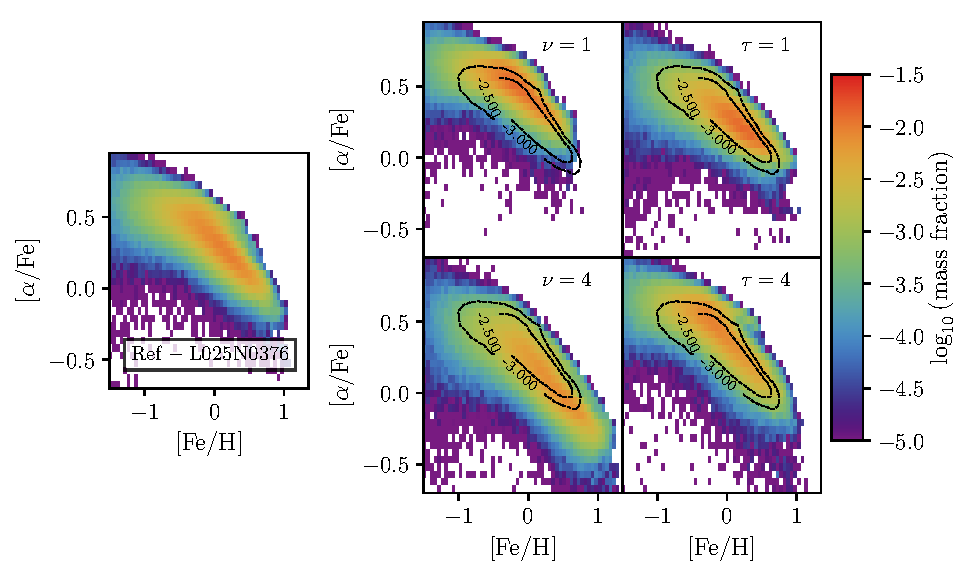
\includegraphics[width=1.\textwidth]{L0100N1504_REFERENCE_disks_4to8_SNIAsubgridvariations.pdf}
\caption[The \afe{}-\feh{} distribution of Milky Way like galaxies in L025N0376 under variations of the SNe feedback sub-grid scheme]{\label{fig:subgrid} The \afe{}-\feh{} distribution of Milky Way like galaxies in simulations of the L025N0376 volume. The left panel shows the distribution realised by the Ref-L025N0376 simulation, whilst the four panels on the right show that from simulations in which a parameter governing the number of Type SNIa per unit stellar mass formed, $\nu$, or the characteristic e-folding timescale of the Type SNIa delay function, $\tau$, has been varied. On these panels, the overlaid black contours are from the Ref-L025N0376 distribution, highlighting the significant changes to the \afe{}-\feh{} distribution induced by these parameter changes.}
\end{figure*}

I briefly examine in this appendix the degree to which variation of the subgrid parameters governing the rate of Type Ia SNe influences the \afe{}-\feh{} distribution of disc stars of Milky Way-like galaxies. I analyse four simulations that adopt the same initial conditions as the Ref-L025N0376 simulation, two of which vary the total number of Type Ia SNe per unit of initial stellar mass formed, adopting $\nu = 1\times 10^{-3}\,{\rm M}_{\odot}^{-1}$ and $\nu = 4\times 10^{-3}\,{\rm M}_{\odot}^{-1}$ (relative to the Reference model, which adopts $\nu = 2\times 10^{-3}\,{\rm M}_{\odot}^{-1}$) , and two of which vary the characteristic e-folding timescale of the Type Ia SNe delay time distribution, adopting $\tau = 1\,{\rm Gyr}$ and $\tau = 4\,{\rm Gyr}$ (where the Reference model assumes $\tau = 2\,{\rm Gyr}$).

I examine the 56 galaxies in the Ref-L025N0376 simulation with $\kappa_\mathrm{co} > 0.4$ and stellar mass in the interval $4 < M_* < 8\times10^{10}\ \mathrm{M_{\odot}}$. I identify the same haloes in the 4 variation runs using the same particle matching technique \citep{2015MNRAS.453L..58S} used to pair haloes with their counterpart in the DMONLY simulation.

The right four panels of Fig. \ref{fig:subgrid} show the \afe{}-\feh{} distribution of these galaxies in the varied simulations as 2-dimensional histograms, with the overlaid contours showing the equivalent distribution from the Reference simulation, shown in its entirety in the left panel. Varying the number of Type Ia SNe per unit stellar mass formed has a significant impact on the distribution, as changing the number of Type Ia SNe also changes the total mass of Fe synthesised per unit stellar mass formed. Decreasing (increasing) the number of Type Ia SNe therefore shifts the distribution upward (downward) to a higher (lower) \afe{}, and truncates the distribution at a lower (higher) \feh{}. The characteristic delay timescale of Type Ia SNe governs the likelihood of gas becoming enriched with the Fe synthesised by Type Ia SNe whose progenitors formed recently. A shorter (longer) delay timescale results in a greater (lesser) fraction of stars forming from Fe-rich gas, inhibiting (aiding) the formation of a high-\afe{} sequence. 

These results indicate that the parameters governing the subgrid implementation of enrichment by Type Ia SNe, which are in general rather poorly constrained, have a tangible impact on the resulting \afe{}-\feh{} distribution of disc stars. This highlights the importance of quantifying these sources of systematic uncertainty, and of ensuring that models used to examine the evolution of galaxy elemental abundances are broadly compatible with orthogonal constraints. As discussed by \citet{2015MNRAS.446..521S}, the values of $\nu$ and $\tau$ adopted by EAGLE were calibrated to ensure that the simulations broadly reproduce the observed evolution of the cosmic Type Ia SNe rate density. 

